\section{Results}
\label{sec:results}

In this section we demonstrate the initial results of the embedding
of two non-rigid registration paradigms each from a different code
base, namely the stationary velocity field transform from the ITKv4
registration framework and the B-spline based registration of the
\elastix{} toolbox.

To demonstrate that the toolbox provides a single interface to 
multiple paradigms we perform a small comparison study on synthetic 
images. The study consists of four experiments, that is, two variations 
of each paradigm: 1) ITKv4 with a stationary velocity field 
transform and 1a) a mean squared difference metric (MSD) or 1b) an ANTs 
neighborhood correlation metric (ANTsC), 2) \elastix{} with a B-spline 
transform and 2a) a MSD metric, or 2b) a 
normalized correlation metric (NC).

Currently, the ITKv4 framework is embedded by three components: a
main component containing the registration framework plus the
transformation model, the MSD metric and the
ANTsC metric. With these components two
similar algorithm networks can be constructed using each of the two
metric components. Currently, \elastix{} is embedded as a monolithic
component in which the choice of metric is considered a setting. This 
illustrates that the framework can deal with different levels of granularity.
The network layouts of the experiments, which are automatically generated by \SuperElastix{} using Graphviz \cite{Gansner:graphviz}, are shown in Figure
\ref{fig:networks}.

\begin{figure}[tb!]
\centering
\begin{tabular}{c@{}c}
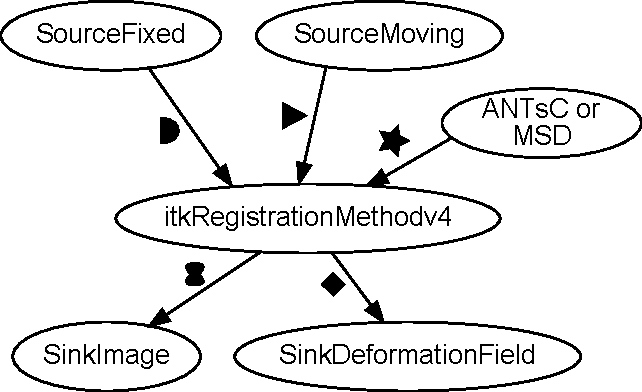
\includegraphics[scale=0.4]{itkv4graph_manual.pdf}  &
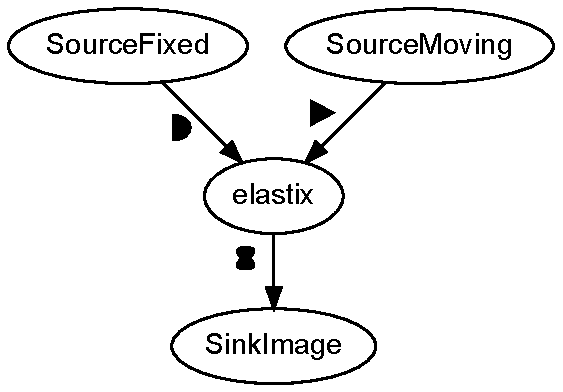
\includegraphics[scale=0.4]{elastixgraph_manual.pdf}
\end{tabular}
\caption{Network configurations for ITKv4 (left) and
\elastix{} (right). Each symbol (\protect
\includegraphics[height=1.2ex]{IFmoon.pdf}
\protect
\includegraphics[height=1.2ex]{IFtriangle.pdf}
\protect
\includegraphics[height=1.2ex]{IFstar.pdf}
\protect
\includegraphics[height=1.2ex]{IFbarbapappa.pdf}
\protect
\includegraphics[height=1.2ex]{IFsquare.pdf}) denotes an interface. The handshake determines that a fixed image interface (\protect
\includegraphics[height=1.2ex]{IFmoon.pdf}) is provided by the SourceFixed component and accepted by the itkRegistrationMethodv4 component.
Currently, the ITKv4 network can be realized with a ANTsC component or an MSD component that both provide a metric interface (\protect
\includegraphics[height=1.2ex]{IFstar.pdf}) that is accepted by the itkRegistrationMethodv4 component. An incorrect configuration, e.g. an ANTsC component connected with a SinkImage component, is detected by the handshake and reported to the user.
}\label{fig:networks}
\end{figure}

For the experiments, synthetic images were chosen such that evident 
differences between the experiments are expected to show up. As 
shown in the left column of Figure \ref{fig:results} both the 
fixed and the moving image have triangular shaped intensity profiles 
with the same maximum intensity and a constant 
but different background. To test the differences due to the 
non-rigid transformation model of the two paradigms, the fixed image 
was constructed to have iso-intensity lines that are elliptical 
whereas they are diamond-shaped in the moving image. Simultaneously, 
the influence of the image similarity metric was tested by setting 
the background intensity value to zero for the fixed image compared 
to a value of one fourth of the maximum for the moving image. For the correlation-based metrics 
an optimal alignment will be where the bases of the intensity shapes 
align, irrespective of the absolute value of the background. In 
contrast, for the squared difference-based metrics, the alignment 
will be optimal if the triangle profile of the moving image aligns 
with the top part of the profile of the fixed image, since this 
minimizes the total absolute difference. 
This is schematically illustrated in Figure \ref{fig:synth_alignment}.
\begin{figure}[!tb]
\centering
\input{synth_alignment.pdf_tex}
\caption{Expected alignment per metric type, with an intensity profile of the fixed image (thin line) and the transformed moving image (thick line).}\label{fig:synth_alignment}
\end{figure}
All registration 
experiments use a multi-resolution approach with 3 levels, using the 
default settings of the toolboxes.

The results of the four experiments are shown in Figure
\ref{fig:results}, where both the deformed moving image and the
resulting deformation field are given. As expected from our
experimental setup the results of each experiment are slightly
different. Both experiments with correlation-based metrics show a
larger cone shape compared to both squared difference-based metrics. 
Between paradigms the differences in
deformation fields can be appreciated. 
For instance, it is clear that the ITKv4 stationary velocity field and the \elastix{} B-spline transformation employ different boundary conditions.

By these experiments we showed that registration algorithms from two
paradigms can be executed and compared using the same interface for passing the
images and algorithm configuration.

\begin{figure}[!tb]
\centering
\begin{tabular}{c@{}c@{}c@{}c@{}c}
Fixed\& &\multicolumn{2}{c}{\elastix{}} & \multicolumn{2}{c}{ITKv4 }\\
Moving  &\multicolumn{2}{c}{B-spline} & \multicolumn{2}{c}{\small Stationary Velocity Field}\\
        &NC & MSD & ANTsC & MSD\\
\hline
  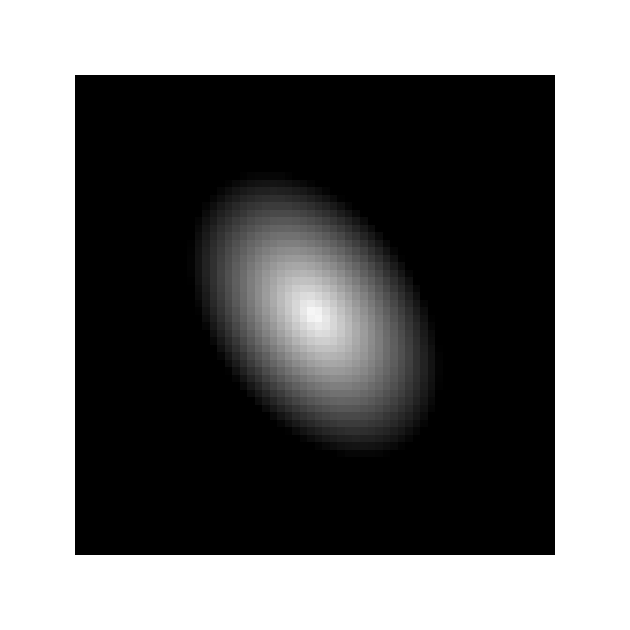
\includegraphics[scale=0.18,trim={5ex 5ex 5ex 5ex},clip=true]{ScriptedImages/fixed.pdf}&
  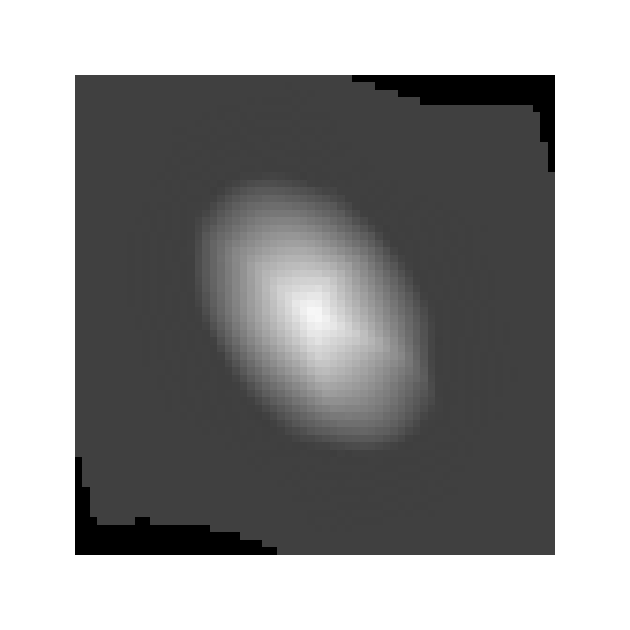
\includegraphics[scale=0.18,trim={5ex 5ex 5ex 5ex},clip=true]{ScriptedImages/elastix_BS_NCC_Image.pdf}&
  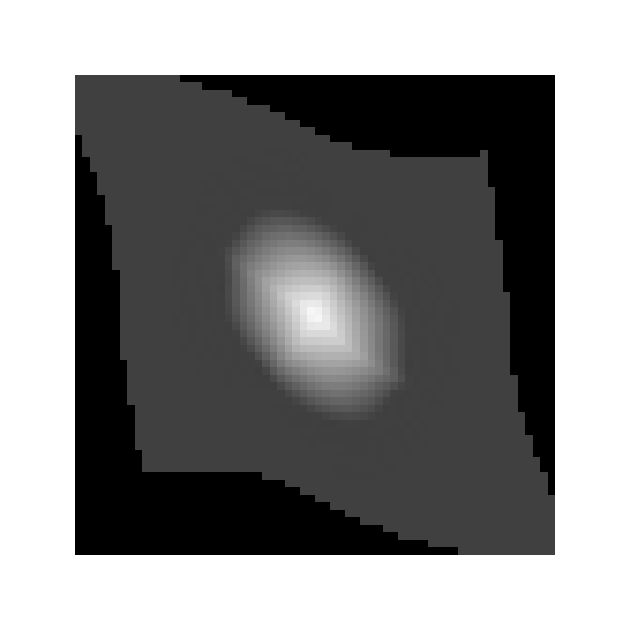
\includegraphics[scale=0.18,trim={5ex 5ex 5ex 5ex},clip=true]{ScriptedImages/elastix_BS_MSD_Image.pdf}&
  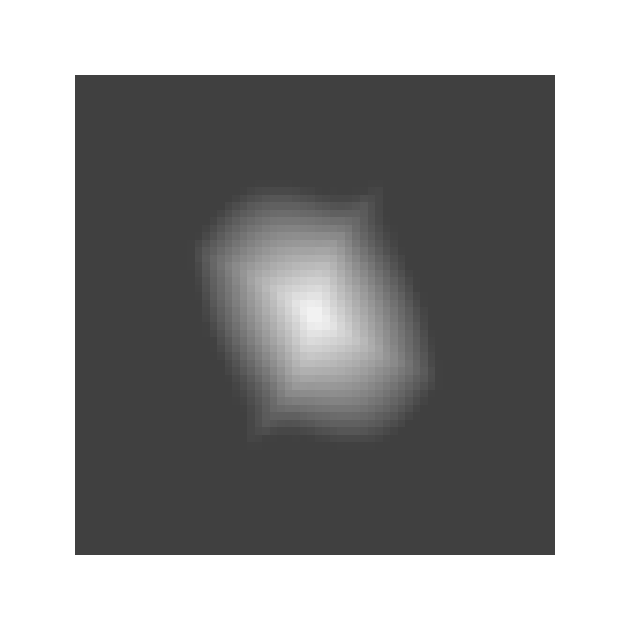
\includegraphics[scale=0.18,trim={5ex 5ex 5ex 5ex},clip=true]{ScriptedImages/itkv4_SVF_ANTSCC_Image.pdf}&
  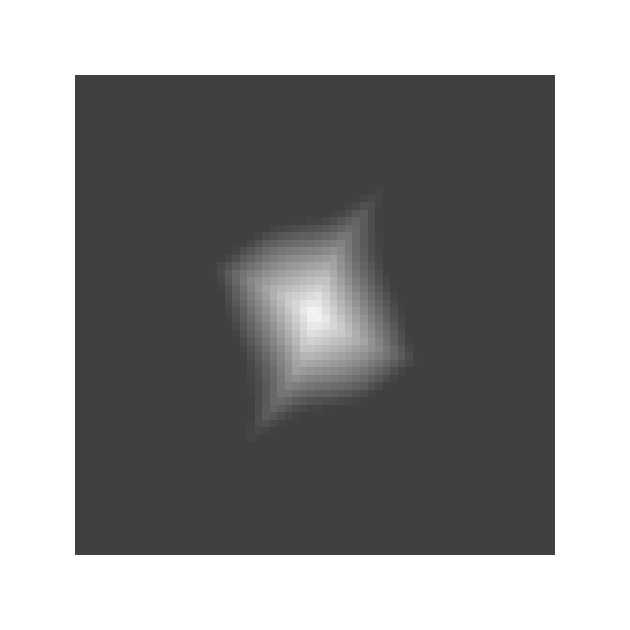
\includegraphics[scale=0.18,trim={5ex 5ex 5ex 5ex},clip=true]{ScriptedImages/itkv4_SVF_MSD_Image.pdf}\\
  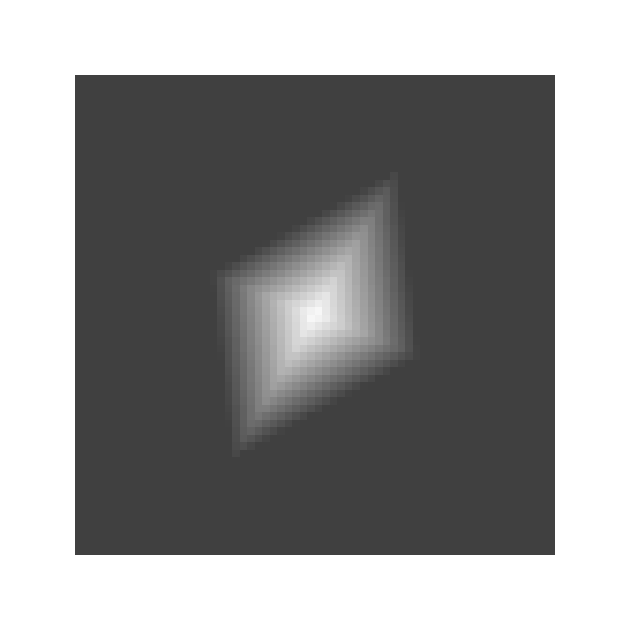
\includegraphics[scale=0.18,trim={5ex 5ex 5ex 5ex},clip=true]{ScriptedImages/moving.pdf}&
  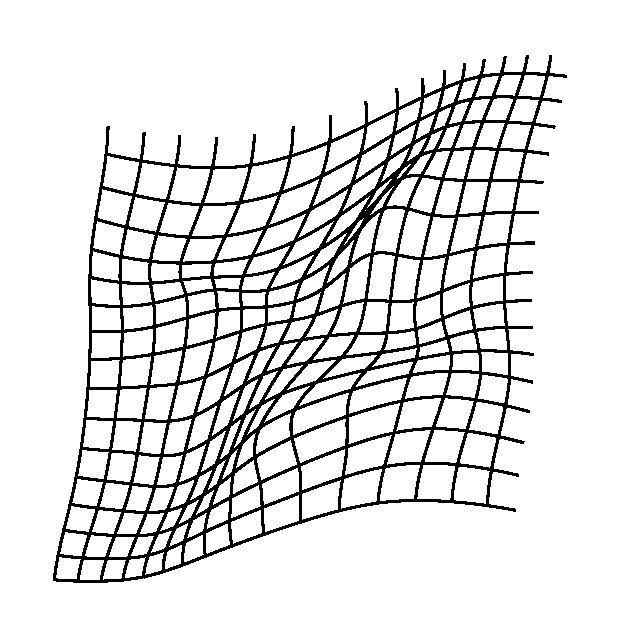
\includegraphics[scale=0.18,trim={5ex 5ex 5ex 5ex},clip=false]{ScriptedImages/elastix_BS_NCC_Displacement.pdf}&
  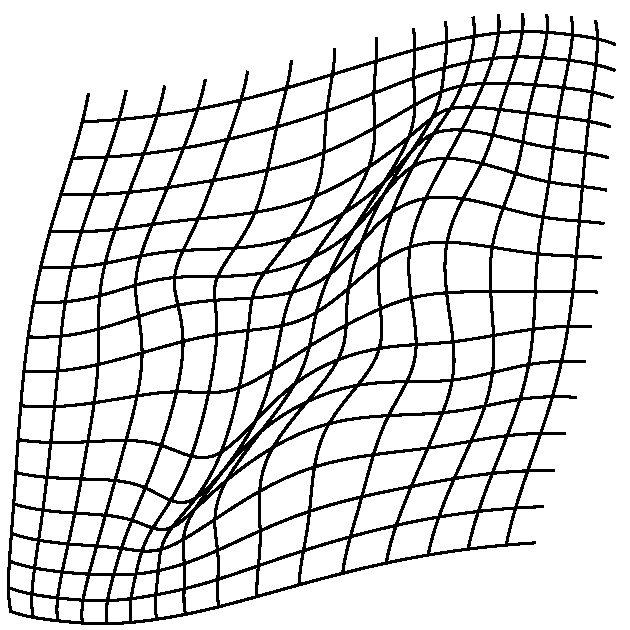
\includegraphics[scale=0.18,trim={5ex 5ex 5ex 5ex},clip=true]{ScriptedImages/elastix_BS_MSD_Displacement.pdf}&
  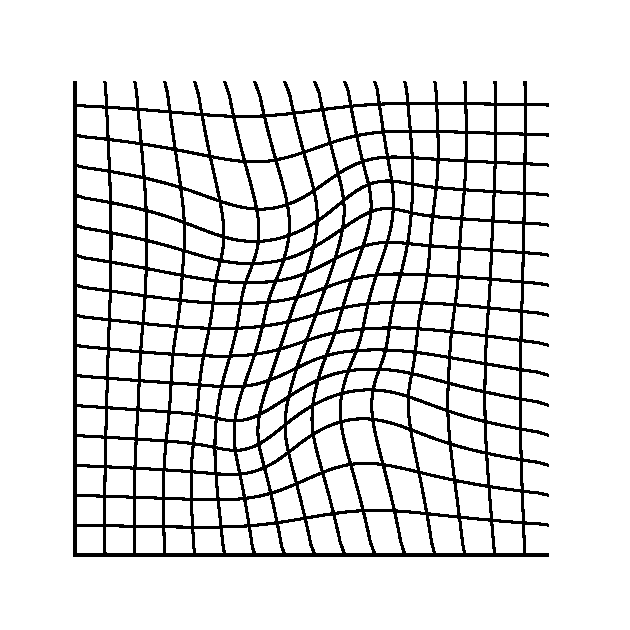
\includegraphics[scale=0.18,trim={5ex 5ex 5ex 5ex},clip=true]{ScriptedImages/itkv4_SVF_ANTSCC_Displacement.pdf}&
  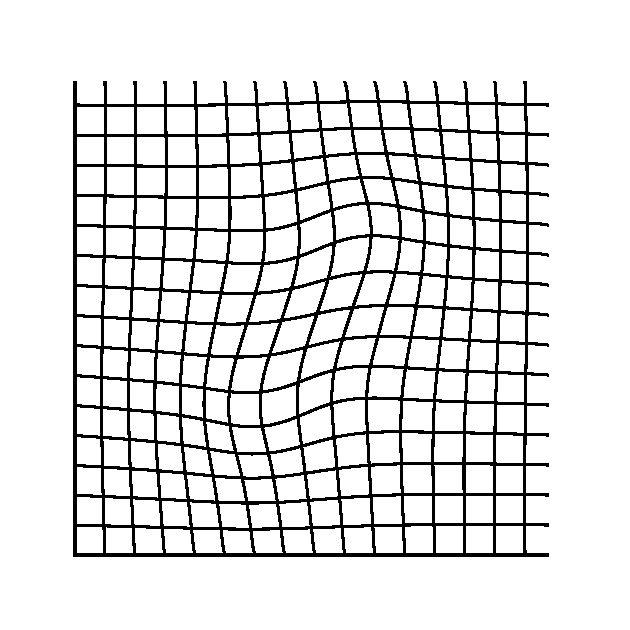
\includegraphics[scale=0.18,trim={5ex 5ex 5ex 5ex},clip=true]{ScriptedImages/itkv4_SVF_MSD_Displacement.pdf}
\end{tabular}
\caption{The fixed and moving image and the results of four
experiments. The resampled moving image and a transformed grid are
shown for each experiment.}\label{fig:results}
\end{figure}
